\documentclass[a4paper]{extarticle}
\usepackage{ctex}
\usepackage{titlesec}
\usepackage{lipsum}
\usepackage{geometry}
\usepackage{amsmath}
\usepackage{biblatex}
\usepackage{booktabs}
\usepackage{caption}
\usepackage{graphicx}
\usepackage{float}
\setCJKmainfont{STSong}[AutoFakeBold,AutoFakeSlant]
\setCJKsansfont{Microsoft YaHei}
\setCJKmonofont{KaiTi}
\setmainfont{Times New Roman}
\setsansfont{Times New Roman}
\setmonofont{Times New Roman}
\linespread{1.5}
\setlength{\parindent}{0pt}
\titleformat{\section}{\bfseries\fontsize{14pt}{\baselineskip}\selectfont}{\thesection}{0.5em}{}
\titleformat{\subsection}{\bfseries\fontsize{10.5pt}{\baselineskip}\selectfont}{\thesubsection}{0.5em}{}
\titleformat{\subsubsection}{\fontsize{10.5pt}{\baselineskip}\selectfont}{\thesubsubsection}{0.5em}{}
\geometry{left=2.5cm,right=2.5cm,top=2.5cm,bottom=2.5cm}
\everymath{\displaystyle}

\begin{document}
    \begin{center}
        \textbf{\fontsize{22pt}{\baselineskip} \selectfont 表面张力数据处理}\\
        \vspace{2em}
        \texttt{\fontsize{14pt}{\baselineskip} \selectfont 作者:刘子墨,学号:PB23000233}\\
    \end{center}
    \section{锥形弹簧的弹性系数}
    逐次在砝码盘内放入砝码,每次增量 0.5g 的砝码,记录升降杆位移读数,得到的数据如下表所示:
    \begin{table}[H]
        \centering
        \caption{锥形弹簧的弹性系数实验数据}
        \begin{tabular}{ccc}
            \toprule
            砝码质量 $m$/g & 砝码重力 $F$/N & 升降杆位移 $x$/cm\\
            \midrule
            0.0 & 0 & 0.99\\
            0.5 & 0.00490 & 1.43\\
            1.0 & 0.00980 & 1.88\\
            1.5 & 0.01469 & 2.37\\
            2.0 & 0.01959 & 2.80\\
            2.5 & 0.02449 & 3.29\\
            3.0 & 0.02939 & 3.74\\
            3.5 & 0.03428 & 4.17\\
            4.0 & 0.03918 & 4.68\\
            4.5 & 0.04408 & 5.12\\
            5.0 & 0.04898 & 5.60\\
            \bottomrule
        \end{tabular}
    \end{table}
    使用Origin软件线性拟合得到:
    \begin{figure}[H]
        \centering
        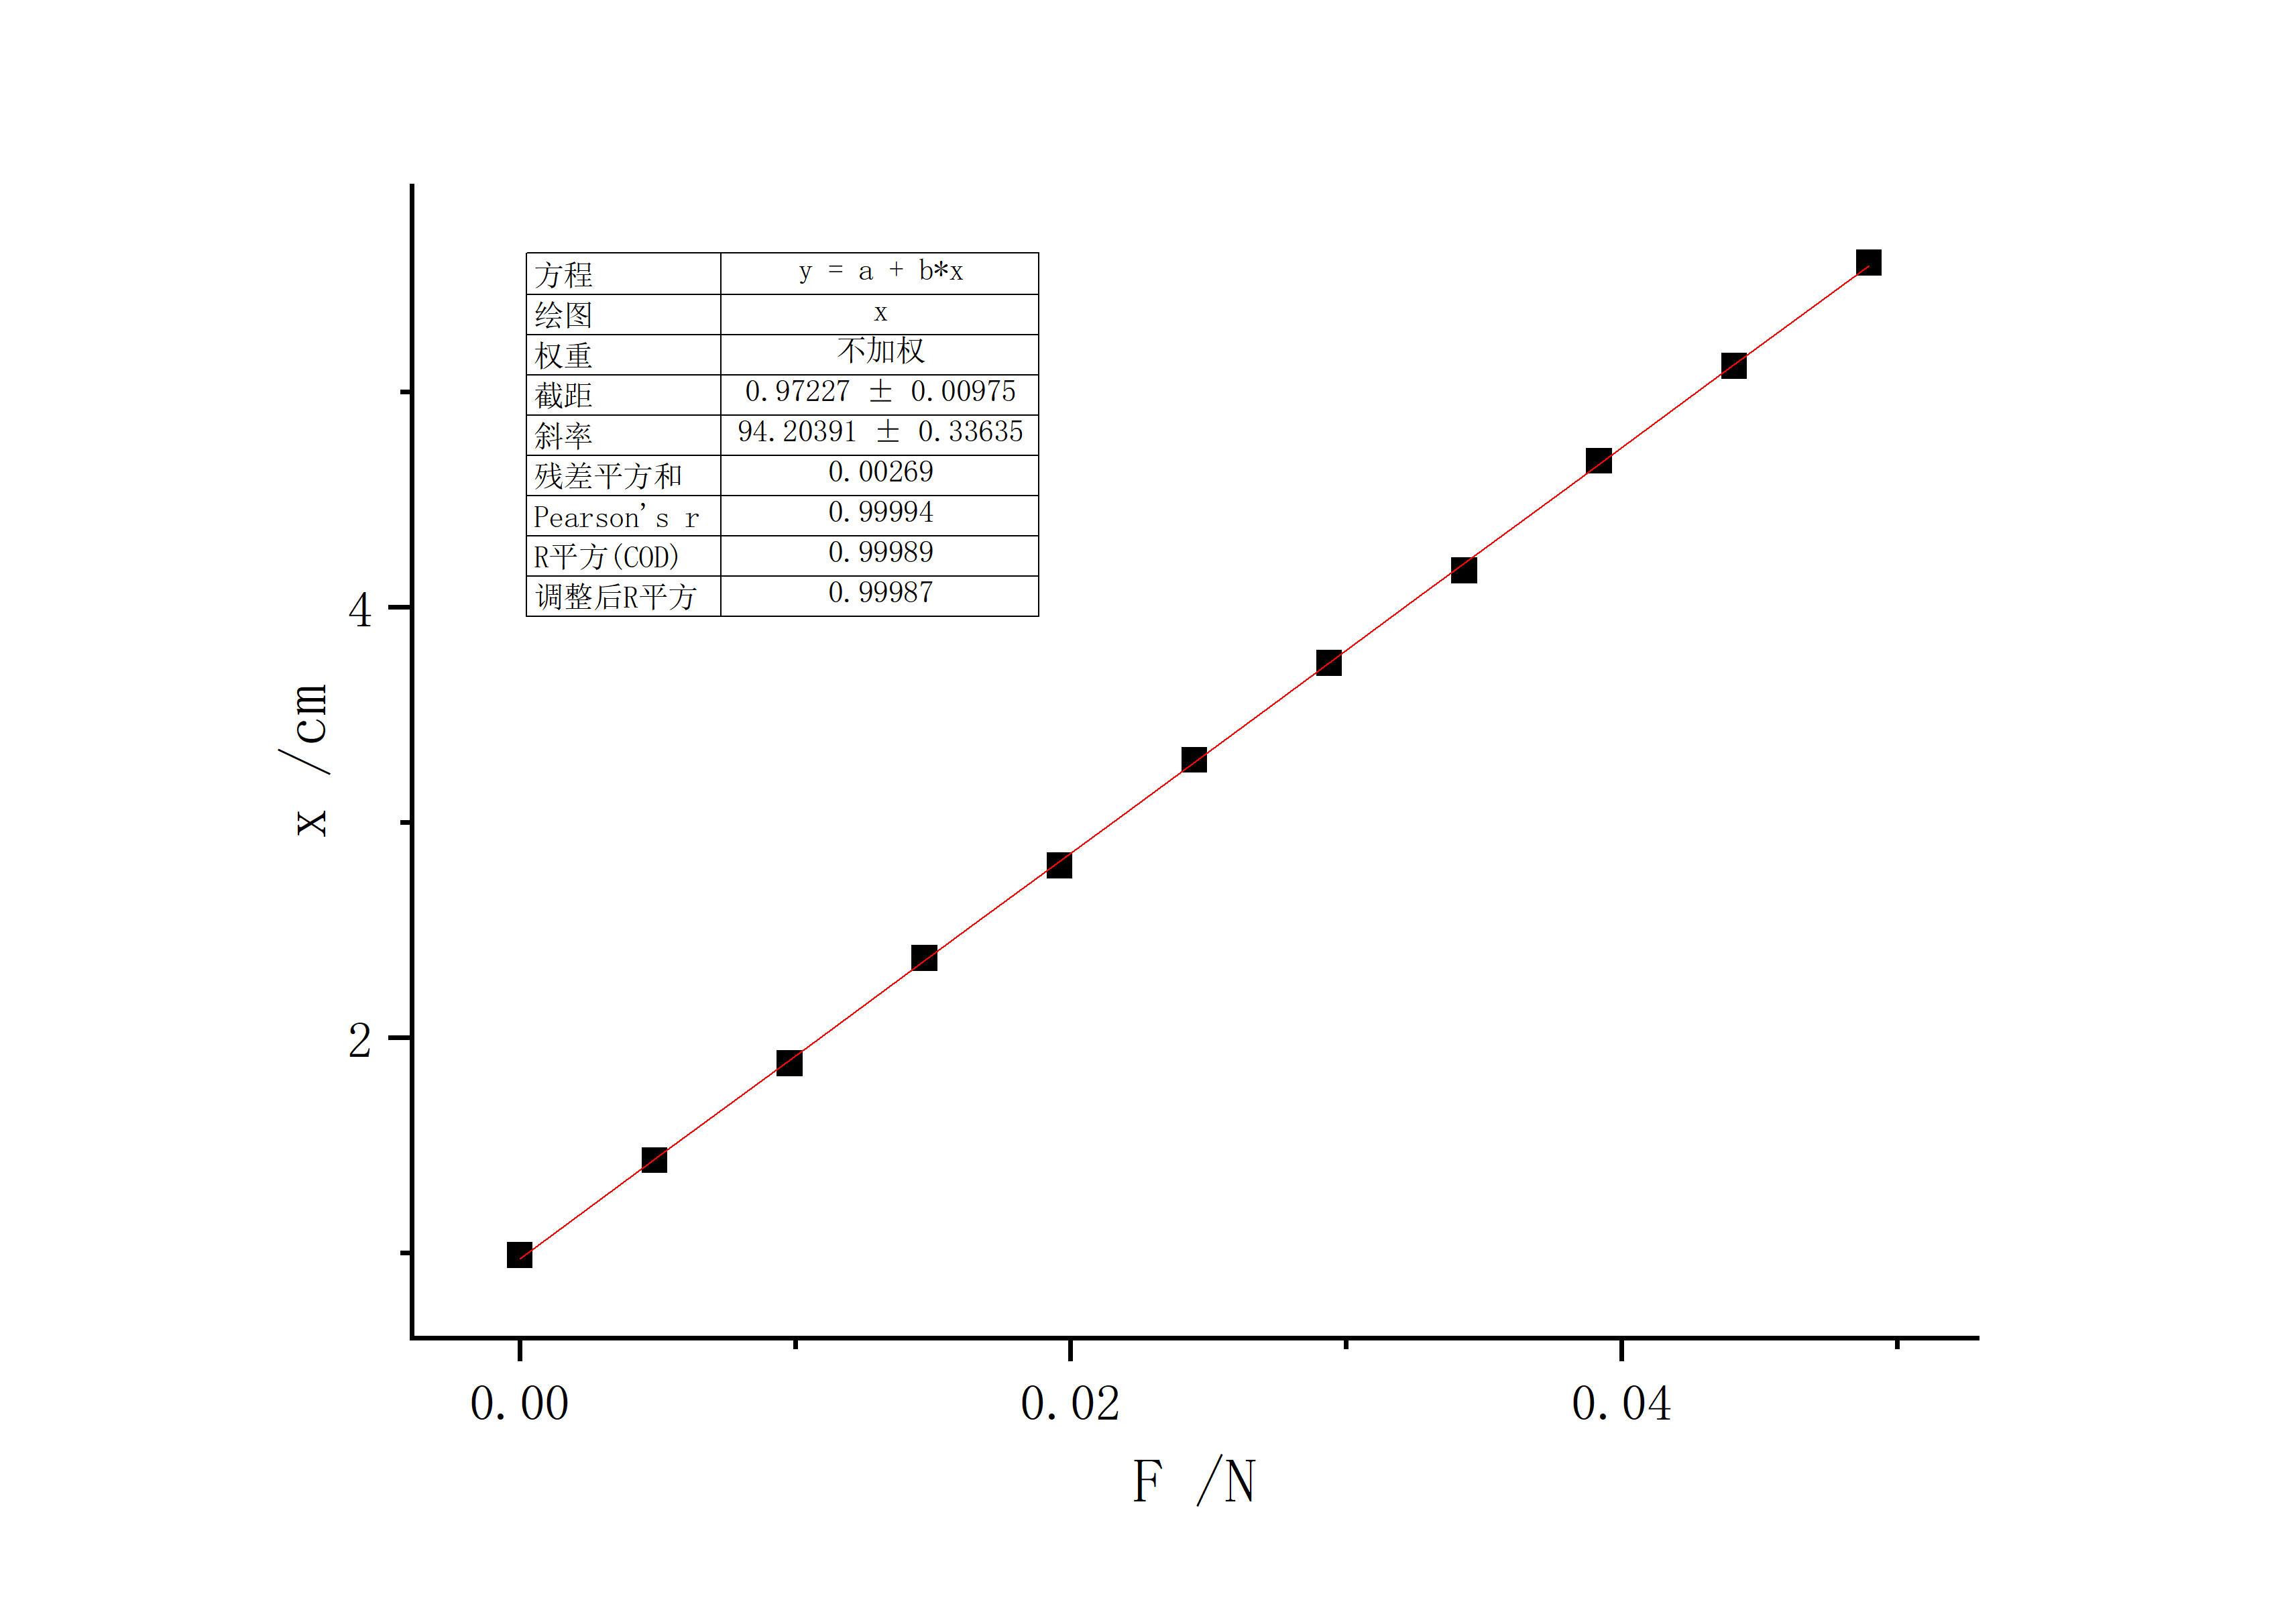
\includegraphics[width=0.8\linewidth]{1.png}
        \caption{砝码重力与位移的实验数据线性拟合}
    \end{figure}
    由图像得到斜率 $0.9420$ m/N ,相关系数为 0.99994 ,即弹簧的弹性系数 $k = 1/0.9420=1.062$ N/m。
    \section{自来水表面张力系数}
    使用拉脱法测量自来水表面张力系数。用钢刻度尺测量使用金属圈直径测量结果如下:
    \begin{table}[H]
        \centering
        \caption{金属圈直径测量数据}
        \begin{tabular}{cc}
            \toprule
            编号 & 金属圈直径 $d$/cm\\
            \midrule
            1 & 3.50\\
            2 & 3.45\\
            3 & 3.50\\
            \midrule
            平均值 & 3.483\\
            \bottomrule
        \end{tabular}
    \end{table}
    使用拉脱法测量时,初始刻度 $l_0 = 0.95$ cm ,重复 5 次,水膜破裂时刻度如下:
    \begin{table}[H]
        \centering
        \caption{水膜破裂时刻度测量数据}
        \begin{tabular}{ccc}
            \toprule
            编号 & 水膜破裂时刻度 $l$/cm & 弹簧伸长量 $\Delta l$ /cm\\
            \midrule
            1 & 2.17 & 1.22\\
            2 & 2.23 & 1.28\\
            3 & 2.21 & 1.26\\
            4 & 2.15 & 1.20\\
            5 & 2.27 & 1.32\\
            \midrule
            平均值 & -- & 1.256\\
            \bottomrule
        \end{tabular}
    \end{table}
    则可以计算出 $F=k\Delta l=1.334\times10^{-2}$ N ,则表面张力系数为:
    \begin{equation*}
        \sigma=\frac{F}{2\pi d}=\frac{1.334\times10^{-2}}{2\pi \times3.483\times10^{-2}}=6.10\times10^{-2} \,\text{N/m}    
    \end{equation*}
    \section{洗洁精表面张力系数}
    使用拉脱法测量洗洁精表面张力系数。用钢刻度尺测量使用金属丝长度测量结果如下:
    \begin{table}[H]
        \centering
        \caption{金属丝长度测量数据}
        \begin{tabular}{cc}
            \toprule
            编号 & 金属丝长度 $s$/cm\\
            \midrule
            1 & 4.45\\
            2 & 4.45\\
            3 & 4.45\\
            \midrule
            平均值 & 4.45\\
            \bottomrule
        \end{tabular}
    \end{table}
    使用拉脱法测量时,初始刻度 $l_0 = 0.80$ cm ,重复 5 次,洗洁精膜破裂时刻度如下:
    \begin{table}[H]
        \centering
        \caption{洗洁精膜破裂时刻度测量数据}
        \begin{tabular}{ccc}
            \toprule
            编号 & 洗洁精膜破裂时刻度 $l$/cm & 弹簧伸长量 $\Delta l$ /cm\\
            \midrule
            1 & 1.04 & 0.24\\
            2 & 1.05 & 0.25\\
            3 & 1.04 & 0.24\\
            4 & 1.05 & 0.25\\
            5 & 1.05 & 0.25\\
            \midrule
            平均值 & -- & 0.246\\
            \bottomrule
        \end{tabular}
    \end{table}
    可以计算出 $F=k\Delta l=2.613\times10^{-3}$ N ,则表面张力系数为:
    \begin{equation*}
        \sigma=\frac{F}{2s}=\frac{2.613\times10^{-3}}{2\times4.45\times10^{-2}}=2.94\times10^{-2} \,\text{N/m}
    \end{equation*}
    \section{不同浓度洗洁精溶液的表面张力关系曲线}
    分别配置4种不同浓度的洗洁精溶液,使用拉脱法测量表面张力系数,得到的数据如下表所示:
    \begin{table}[H]
        \centering
        \caption{不同浓度洗洁精溶液的表面张力系数}
        \begin{tabular}{cccc}
            \toprule
            水与洗洁精体积比 & 初始刻度 $l_0$/cm & 破裂时刻度 $l$/cm & 弹簧伸长量 $\Delta l$/cm\\
            \midrule
            400:1 & 0.80 & 1.04 & 0.24\\
            400:1.6 & 0.86 & 1.11 & 0.25\\
            400:2.6 & 0.83 & 1.09 & 0.26\\
            400:3.6 & 0.82 & 01.09 & 0.27\\
            \bottomrule
        \end{tabular}
    \end{table}
    可以按照上述方法计算出不同浓度洗洁精溶液的表面张力系数:
    \begin{equation*}
        \begin{aligned}
            \sigma_{400:1} &= \frac{k\Delta l}{2s} =\frac{1.062\times0.24\times10^{-2}}{2\times4.45\times10^{-2}}=2.86\times10^{-2} \,\text{N/m}\\
            \sigma_{400:1.6} &= \frac{k\Delta l}{2s} =\frac{1.062\times0.25\times10^{-2}}{2\times4.45\times10^{-2}}=2.98\times10^{-2} \,\text{N/m}\\
            \sigma_{400:2.6} &= \frac{k\Delta l}{2s} =\frac{1.062\times0.26\times10^{-2}}{2\times4.45\times10^{-2}}=3.10\times10^{-2} \,\text{N/m}\\
            \sigma_{400:3.6} &= \frac{k\Delta l}{2s} =\frac{1.062\times0.27\times10^{-2}}{2\times4.45\times10^{-2}}=3.22\times10^{-2} \,\text{N/m}\\            
        \end{aligned}
    \end{equation*}
    将得到表面张力与体积比拟合:
    \begin{figure}[H]
        \centering
        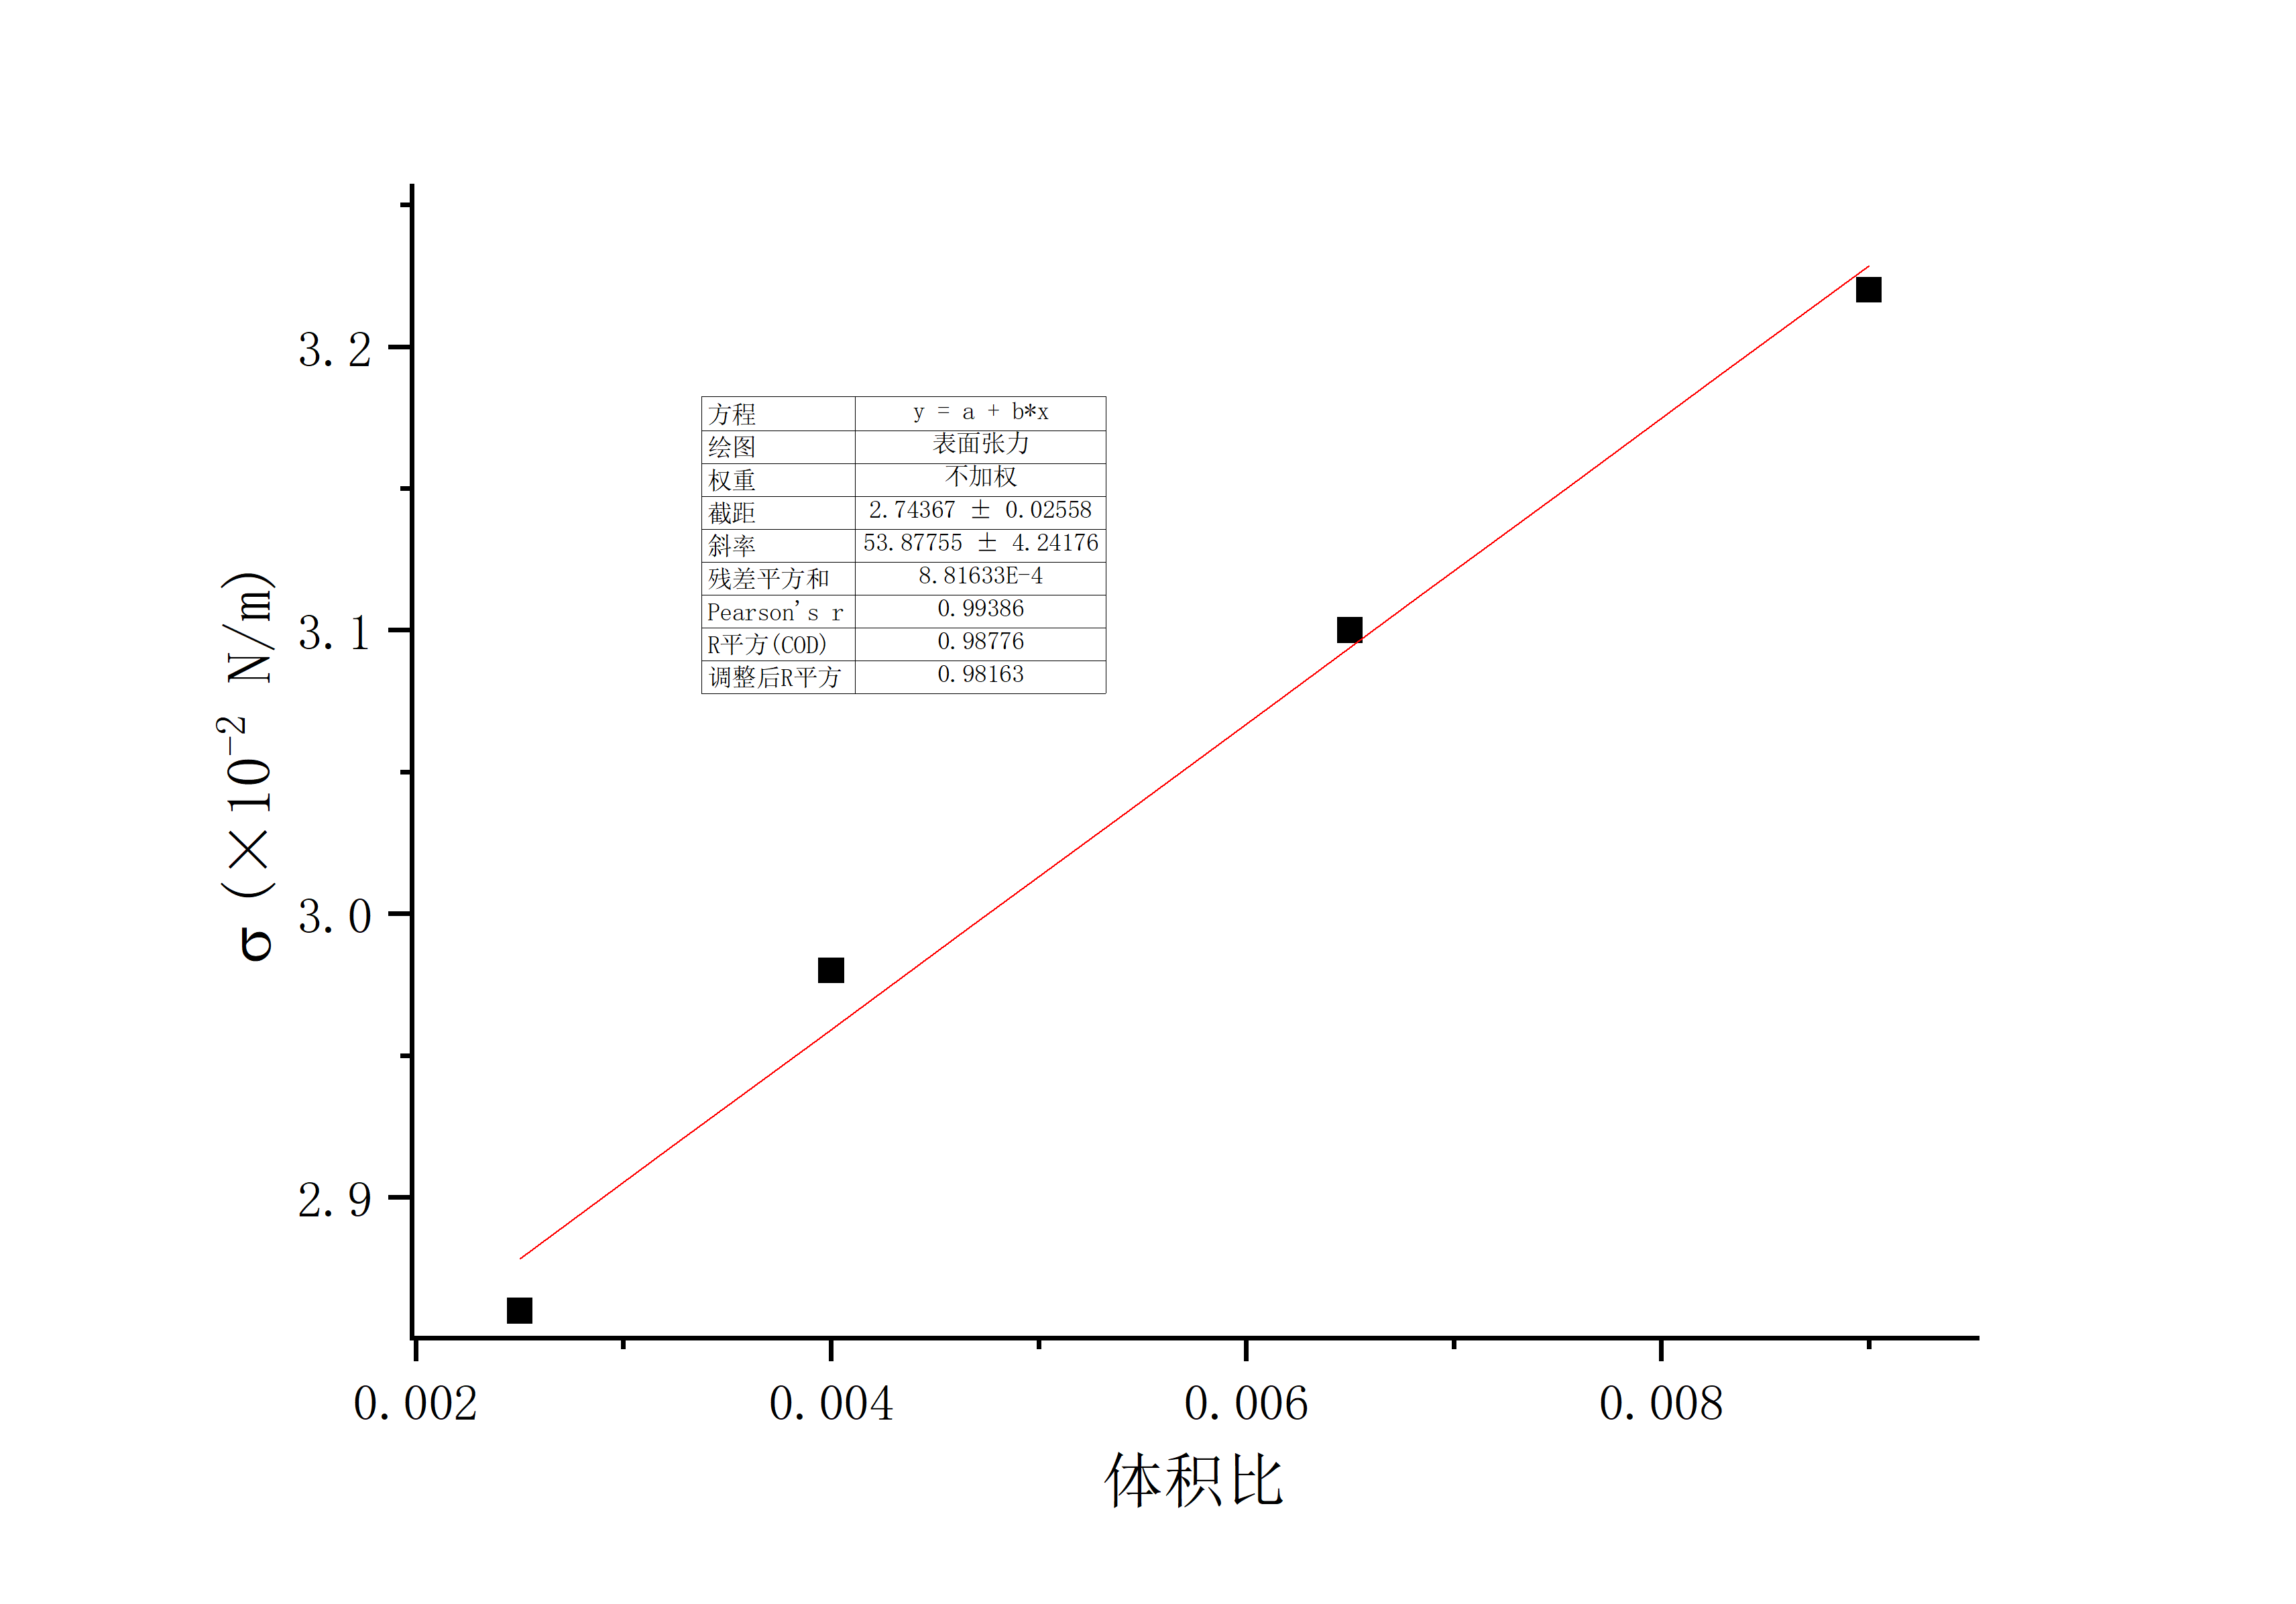
\includegraphics[width=0.8\linewidth]{2.png}
        \caption{洗洁精溶液表面张力与其浓度的线性拟合}
    \end{figure}
    由图可知,洗洁精溶液表面张力与其体积分数大体呈线性关系,但是实验中洗洁精浓度梯度过小,测量的弹簧伸长量间隔过小,结果可能不准确。
    \newpage
    \section*{附录}
    老师签字的实验数据:
    \begin{figure}[H]
        \centering
        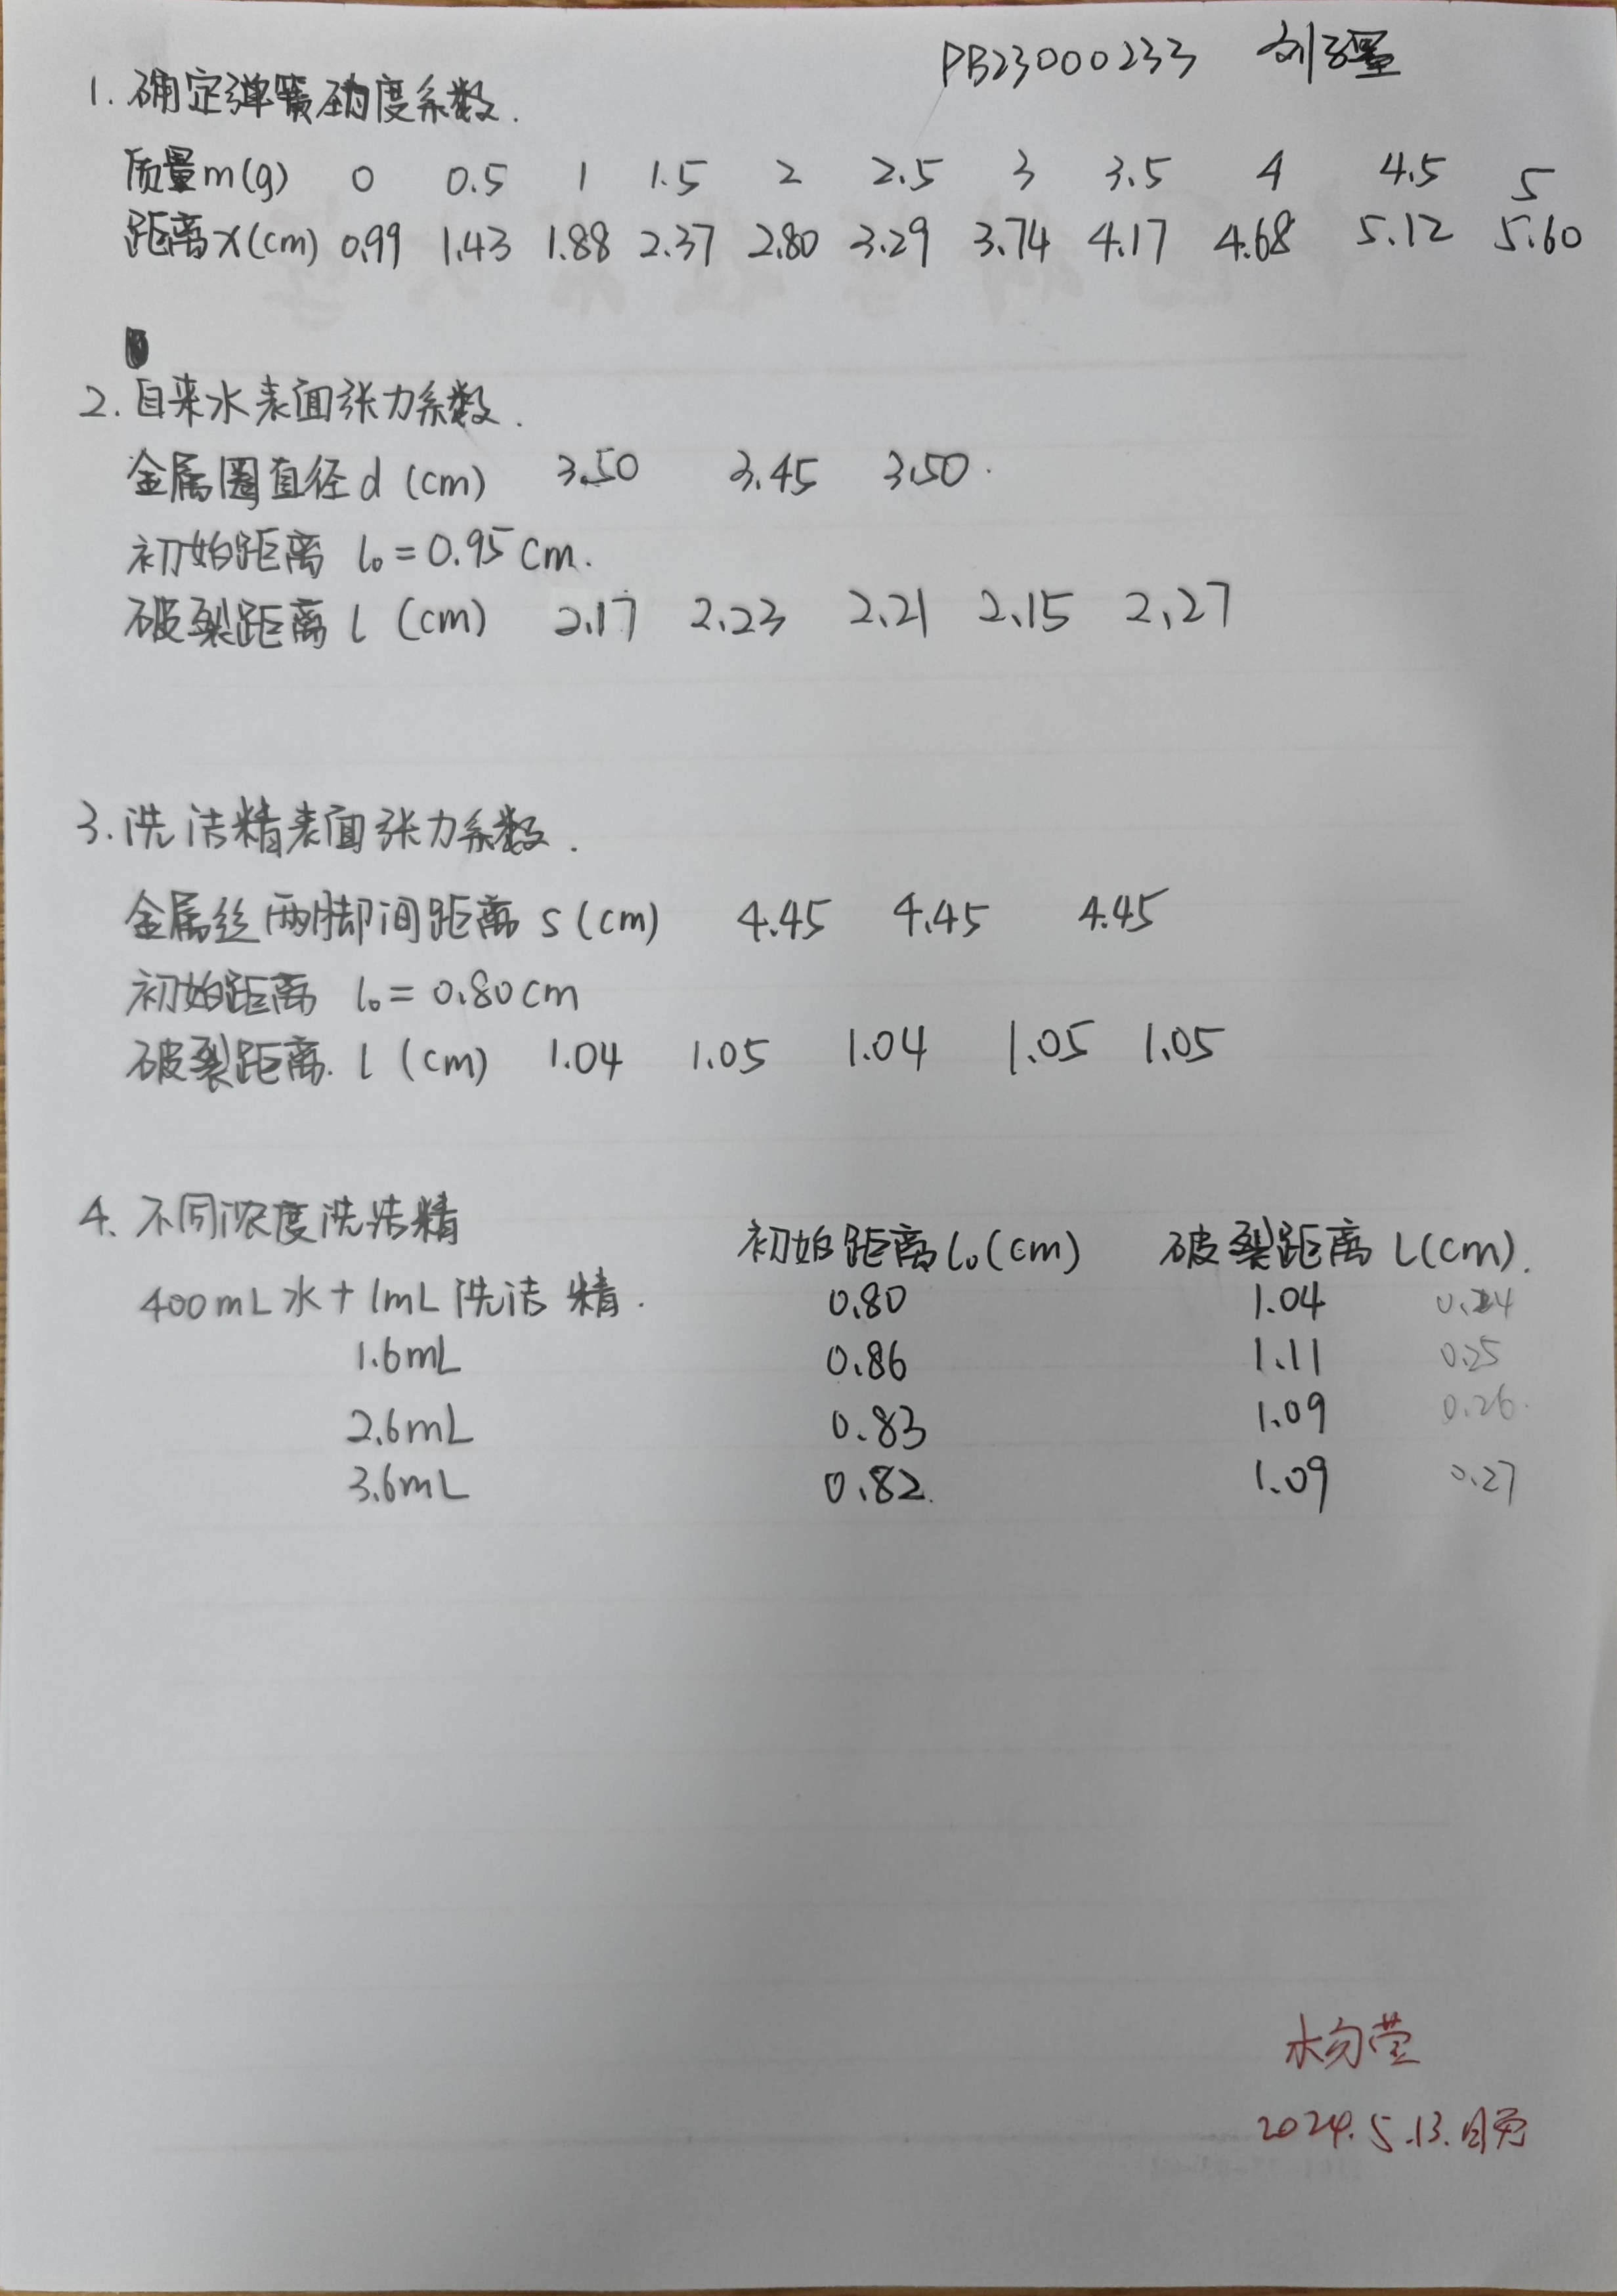
\includegraphics[width=0.98\linewidth]{shuju.jpg}
    \end{figure}
\end{document}
